\documentclass{article}
\usepackage[utf8]{inputenc}
\usepackage{listings}
\usepackage{color} %red, green, blue, yellow, cyan, magenta, black, white
\usepackage{graphicx}
\definecolor{mygreen}{RGB}{28,172,0} % color values Red, Green, Blue
\definecolor{mylilas}{RGB}{170,55,241}
\usepackage[margin=1in]{geometry}

\lstset{language=Matlab,%
    %basicstyle=\color{red},
    breaklines=true,%
    morekeywords={matlab2tikz},
    keywordstyle=\color{blue},%
    morekeywords=[2]{1}, keywordstyle=[2]{\color{black}},
    identifierstyle=\color{black},%
    stringstyle=\color{mylilas},
    commentstyle=\color{mygreen},%
    tabsize=2,
    showstringspaces=false,%without this there will be a symbol in the places where there is a space
    numbers=left,%
    numberstyle={\tiny \color{black}},% size of the numbers
    numbersep=9pt, % this defines how far the numbers are from the text
    emph=[1]{for,end,break},emphstyle=[1]\color{red}, %some words to emphasise
    %emph=[2]{word1,word2}, emphstyle=[2]{style},    
}

\title{Pattern Recognition Assignment 1}
\author{James Jackson}
\date{November 2015}

\begin{document}

\maketitle

\section*{Question 1}
\lstinputlisting{pttrnAss1_1.m}
For output please see figure~\ref{fig:digits}
\begin{figure}
\centering
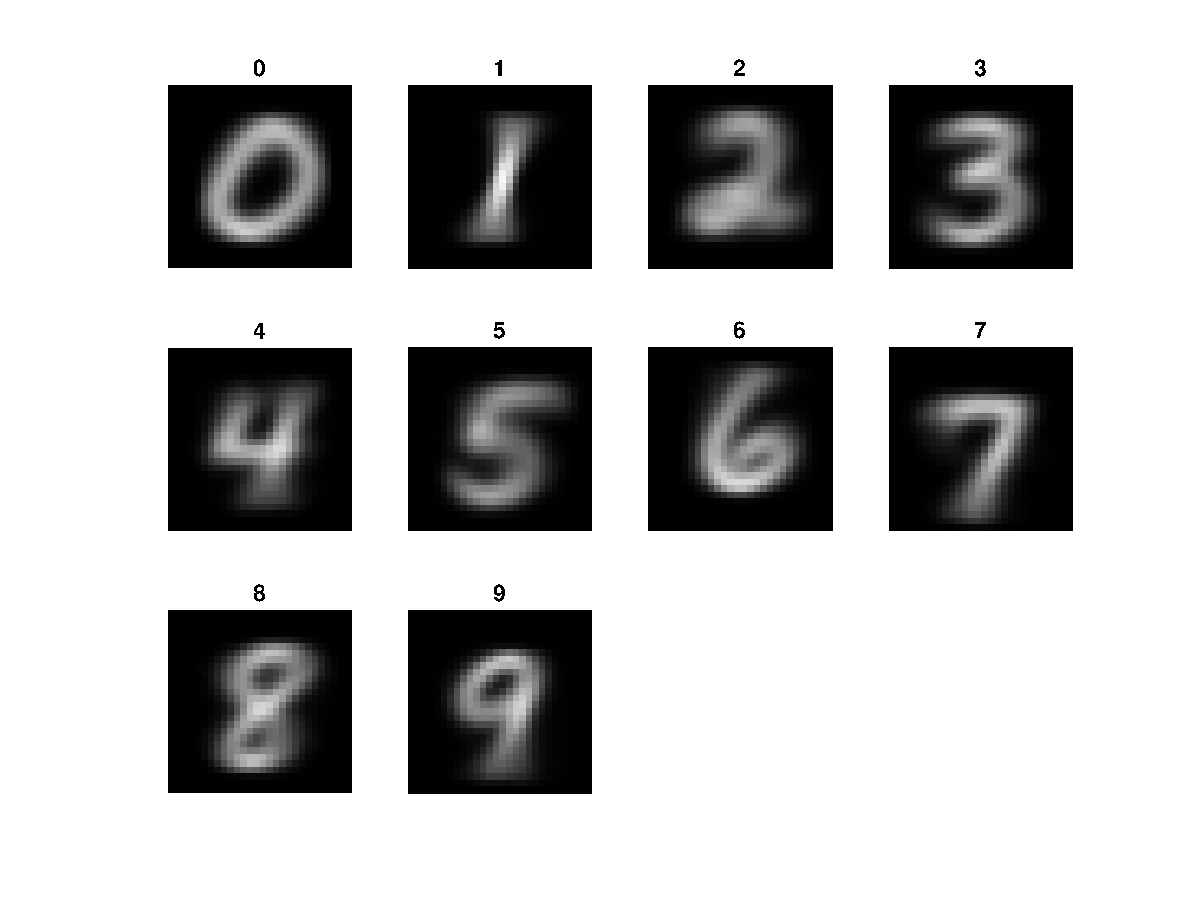
\includegraphics[width=\textwidth]{digits}
\caption{Average digit visualisation}
\label{fig:digits}
\end{figure}

\pagebreak

\section*{Question 2}
\lstinputlisting{pttrnAss1_2.m}
\pagebreak
\section*{Question 3}
\lstinputlisting{pttrnAss1_3.m}
\lstinputlisting{MyNMC.m}
Using the given classifier indicates that the digit 1 is a more distinct as it will have a lower aspect ratio and lower proportion of black as seen by figure~\ref{fig:3a}
\begin{figure}
\centering
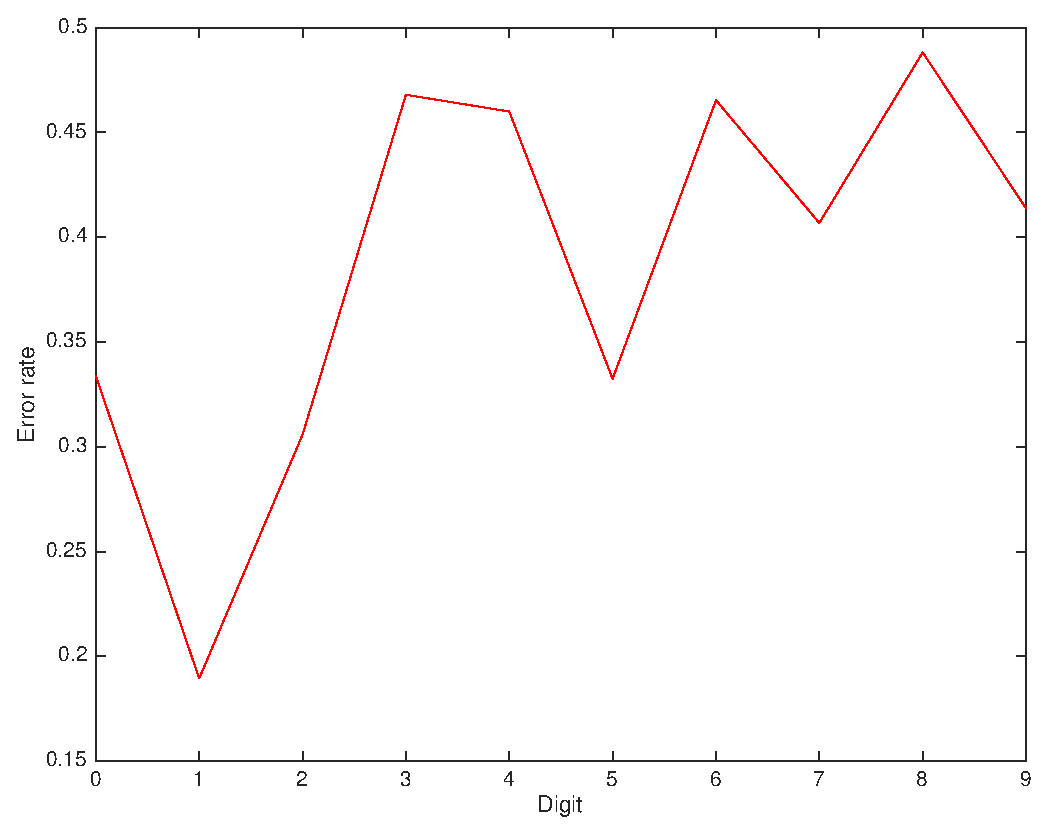
\includegraphics[width=\textwidth]{3a}
\caption{Plot of given classifier error (3a)}
\label{fig:3a}
\end{figure}

In task 3c we use the MyNMC classifier to classify the data and we notice that the error plot (figure~\ref{fig:3c}) it very similar to that of the given classifier which leads to the conclusion that it is an NMC classifier. THe slight differences in error is down to the fact that in figure~\ref{fig:3c} a leaveone out NMC is being used, whereas in figure~\ref{fig:3a} the classifier is being trained on all of the data.

Actual error rates below.

\begin{lstlisting}
    3a        3c
    0.3338    0.3338
    0.1894    0.1894
    0.3058    0.3058
    0.4680    0.4680
    0.4600    0.4600
    0.3324    0.3324
    0.4654    0.4654
    0.4068    0.4068
    0.4882    0.4882
    0.4138    0.4138
\end{lstlisting}

\begin{figure}
\centering
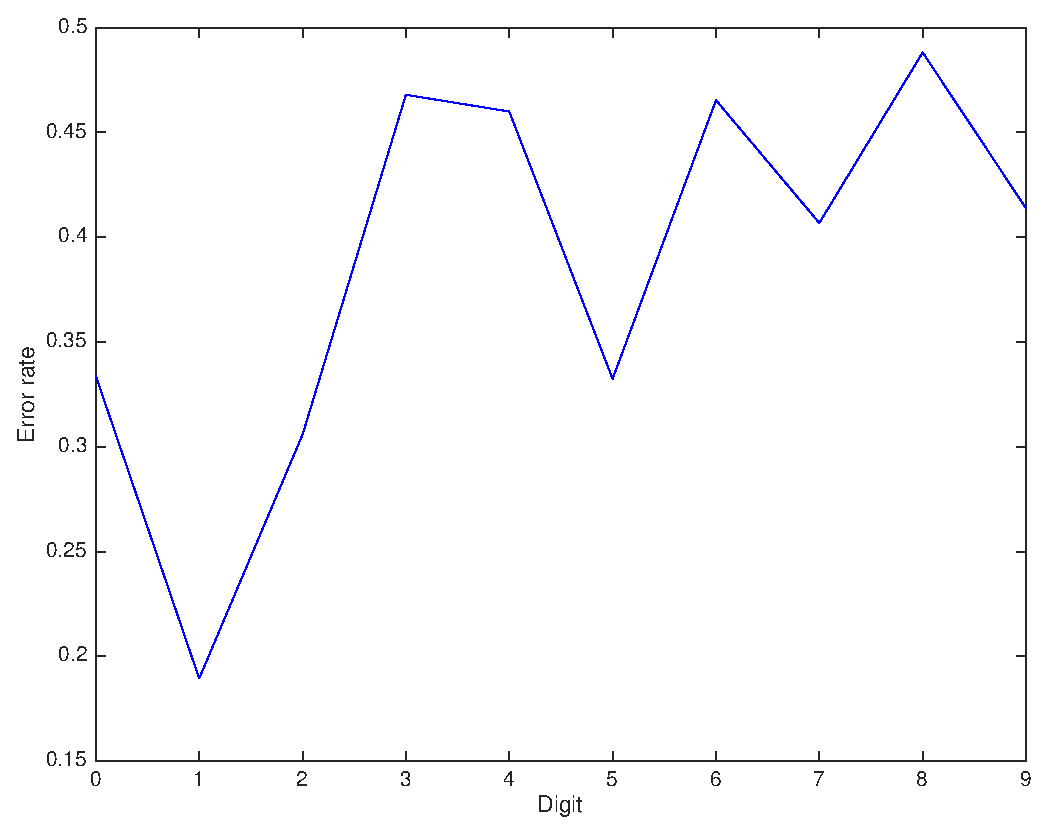
\includegraphics[width=\textwidth]{3c}
\caption{Plot of given classifier error (3c)}
\label{fig:3c}
\end{figure}

\pagebreak

\section*{Question 4}
\lstinputlisting{pttrnAss1_4.m}

When not considering aspect ratio and ink amount the NMC classifier returns different results in terms of error rate, there are differing peaks but better overall error rate as seen in figure~\ref{fig:plot4}

Error rates

\begin{lstlisting}
    Original  Threshold
    0.0522    0.0528
    0.0646    0.0636
    0.0786    0.0770
    0.1002    0.0974
    0.1268    0.1262
    0.1780    0.1774
    0.0666    0.0660
    0.0784    0.0780
    0.1206    0.1220
    0.1828    0.1816
\end{lstlisting}

\begin{figure}
\centering
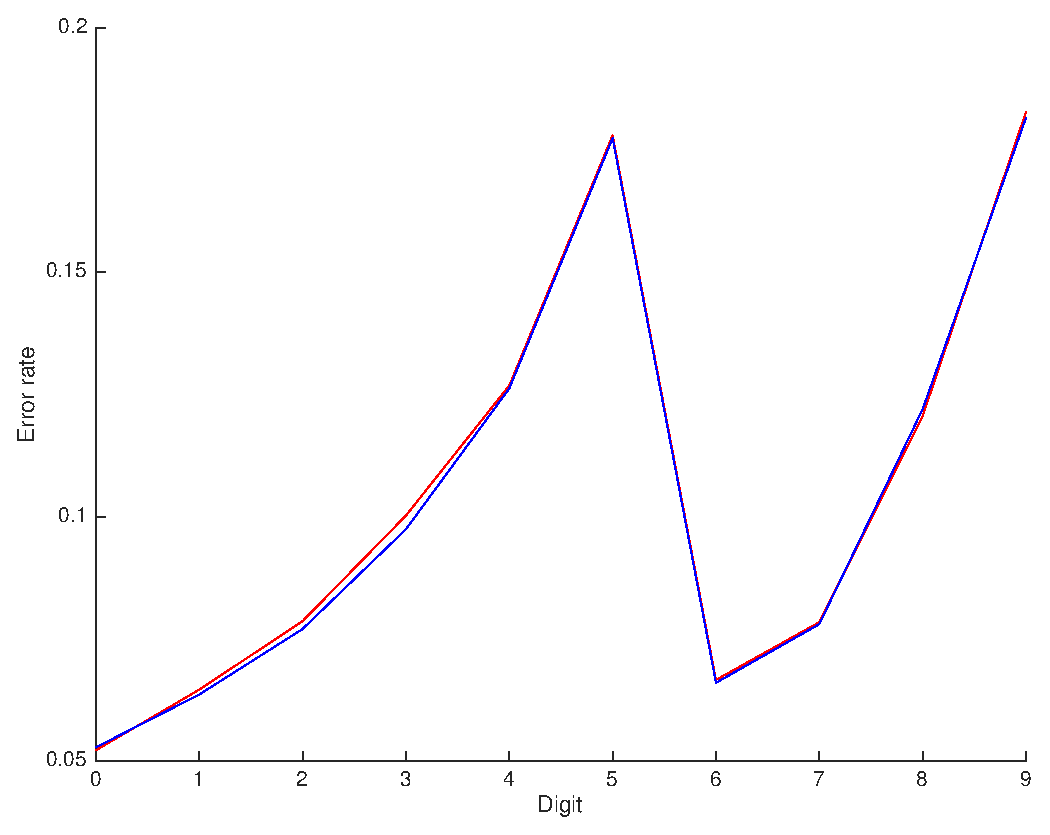
\includegraphics[width=\textwidth]{plot4}
\caption{Plot of given classifier error (4)}
\label{fig:plot4}
\end{figure}


\pagebreak
\section*{Question 5}
\lstinputlisting{MyRoc.m}


\pagebreak
\section*{Question 6}
\lstinputlisting{pttrnAss1_6.m}
For output, see plot in figure~\ref{fig:plot6} The closest points to [0,1] in each case are
\begin{lstlisting}
    Aspect Ratio
    0.8315    0.8633
    Proportion
    0.8763    0.8204

\end{lstlisting}

\begin{figure}
\centering
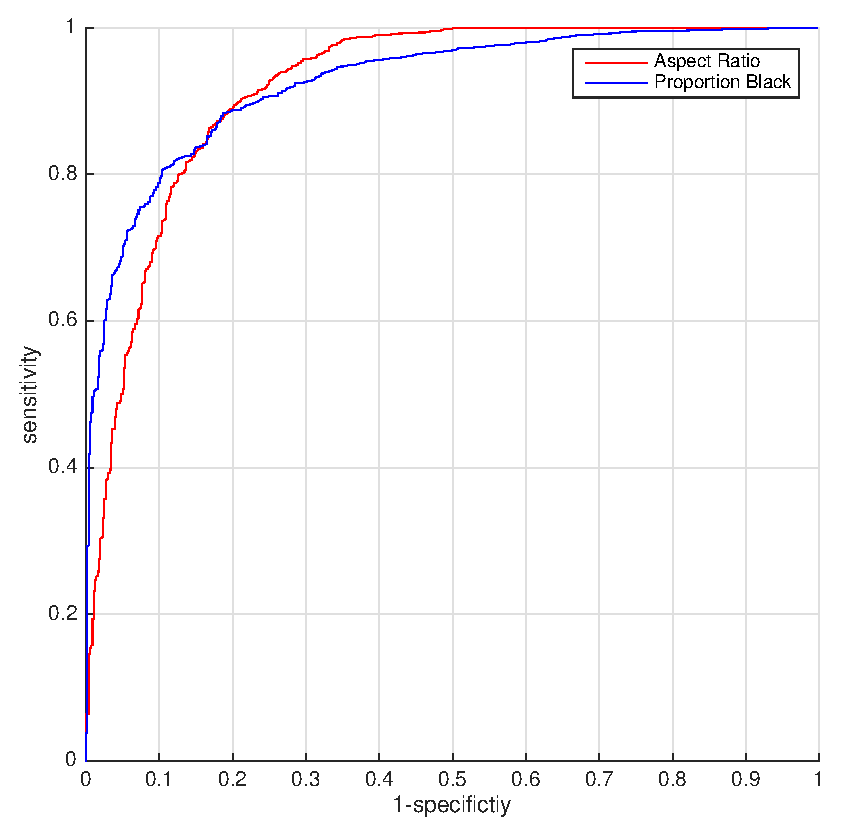
\includegraphics[width=\textwidth]{plot6}
\caption{Plot rock curve for aspect ratio and proportion (6)}
\label{fig:plot6}
\end{figure}


\pagebreak
\section*{Question 7}
\lstinputlisting{pttrnAss1_7.m}
\pagebreak
Confusion matrix

\begin{lstlisting}
   424     0     2     1     0    46    16     1     2     2
     0   537     2     3     0     6     2     0     8     0
    10    32   422    17    20     3    15     9    15     2
     4    16    13   375     1    29     4     3    25    10
     0     7     2     0   393     0     4     1     4    66
     7    37     4    56     5   320    11     3     7    19
     9    16     6     0    15    17   450     0     3     0
     1    28     4     0     9     2     1   422     6    33
     4    21     4    48     3    15     4     1   358    19
     6    11     3     9    48     4     1    19     8   369
\end{lstlisting}

The accuracy for the ensemble is around $ 0.81 $ and the single NMC has a similar accuracy at around $ 0.81 $. 
\end{document}
